
\documentclass{article}
\author{fblazco}
\title{IIC2343}
\usepackage{amsmath}
\usepackage{graphicx}
\begin{document}
	\maketitle
    \section{Clase 1}
    \begin{enumerate}
        \item \textbf{Fecha Evaluaciones}
    \end{enumerate}    
    \section{Clase 2}
    \section{Clase 3}
    \begin{enumerate}
        \subsection{Compuertas}
        \item La compuerta NOT es un relee con salida not(A), y entradas A y corriente
        \item Lacompuerta OR se compone de 2 relee juntos (hacer tablita)
        \item La compuerta AND son dos relee consecutivos (en secuencia) donde el segundo esta conectado a la corriente del primero
        \item Propuesto: Definir \begin{enumerate}
            \item XOR, 
            \item   NAND 
            \item NOR 
            \item XNOR
        \end{enumerate}  usando reeles
    \end{enumerate}
        \subsection{HALF-ADDER}
        \begin{enumerate}
            \item Recibe dos señales de entrada y entrega 2 señales de salida, el Carry y el S (permite sumas de 1 bit sin tomar en cuenta el Carry)
           \item \begin{figure}
                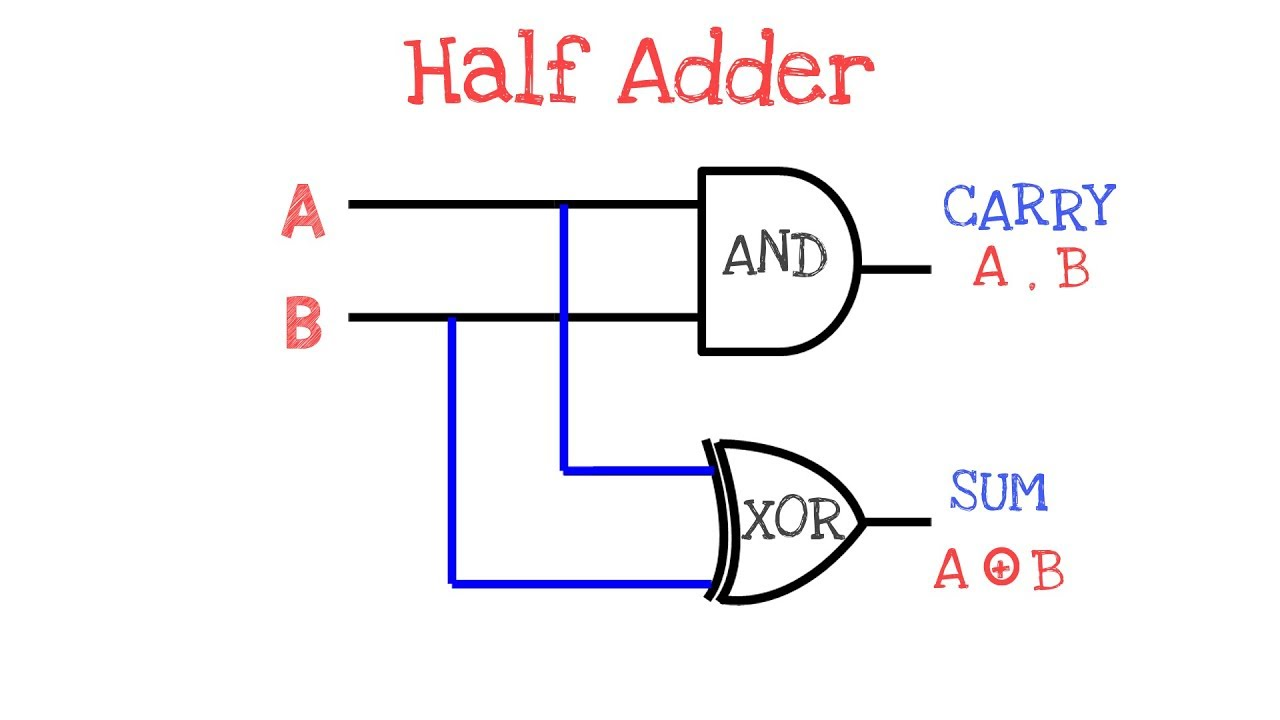
\includegraphics[width=300px]{halfadder.jpg}
                \caption{HF}
                \label{fig:HALF-ADDER}
            \end{figure}
        \end{enumerate}
        
        \subsection{FULL-ADDER}
            \begin{enumerate}
                \item Un full adder esta compuesto de 2 HALF-ADDER, esto nos permite realizar la suma entre 2 bits, considerando el Carry
            \end{enumerate}
             \begin{figure}
                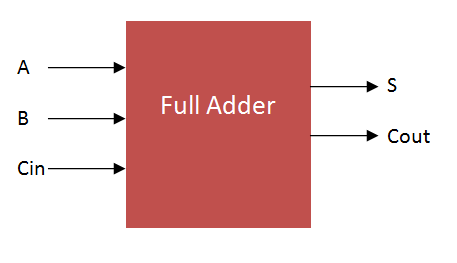
\includegraphics[width=250px]{fulladder.png}
                \caption{HF}
                \label{fig:Full-adder}
            \end{figure}
        \subsection{Sumador de 4bits}
        \begin{figure}
            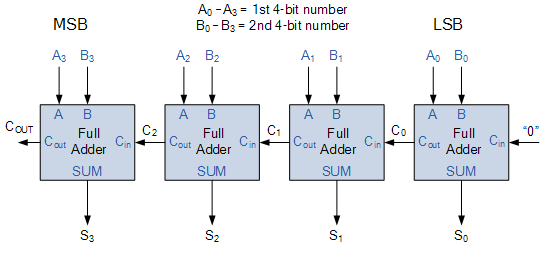
\includegraphics[width=300px]{sumador4bits.png}
            \caption{HF}
            \label{fig:Sumador 4bits}
        \end{figure}
        \begin{enumerate}
            \item Concatenando n full-adders, podemos crear sumadores de n bits, respetando el acarreo
            \item 
        \end{enumerate}
\end{document}  



